
\subsubsection{5.1 RQ1: Alignment Fingerprint Existence (h-e1)}

\textbf{The DPO/SFT alignment fingerprint is confirmed at statistically significant accuracy.}
A k-NN (k=1) LOO-CV classifier correctly identifies the alignment strategy of 10 out
of 12 models (83.3\% accuracy), with permutation test p=0.031 (1000 shuffles). Both
thresholds are exceeded: accuracy (83.3\% vs $\geq 67$\% required) and significance (p=0.031
vs $p\leq 0.05$ required). Alignment strategy is recoverable from a 4D benchmark profile
without any access to training data, preference datasets, or model weights.

\begin{table}[htbp]
\centering
\resizebox{\columnwidth}{!}{%
\begin{tabular}{llll}
\toprule
Metric & Value & Threshold & Status \\
\midrule
LOO-CV accuracy (k=1) & **83.3\%** (10/12) & $\geq 67$\% & PASS \\
Permutation p-value & **p=0.031** & $\leq 0.05$ & PASS \\
\bottomrule
\end{tabular}
}
\end{table}

\textbf{Table 4: Classification results (h-e1 gate).}

\begin{figure}[htbp]
\centering
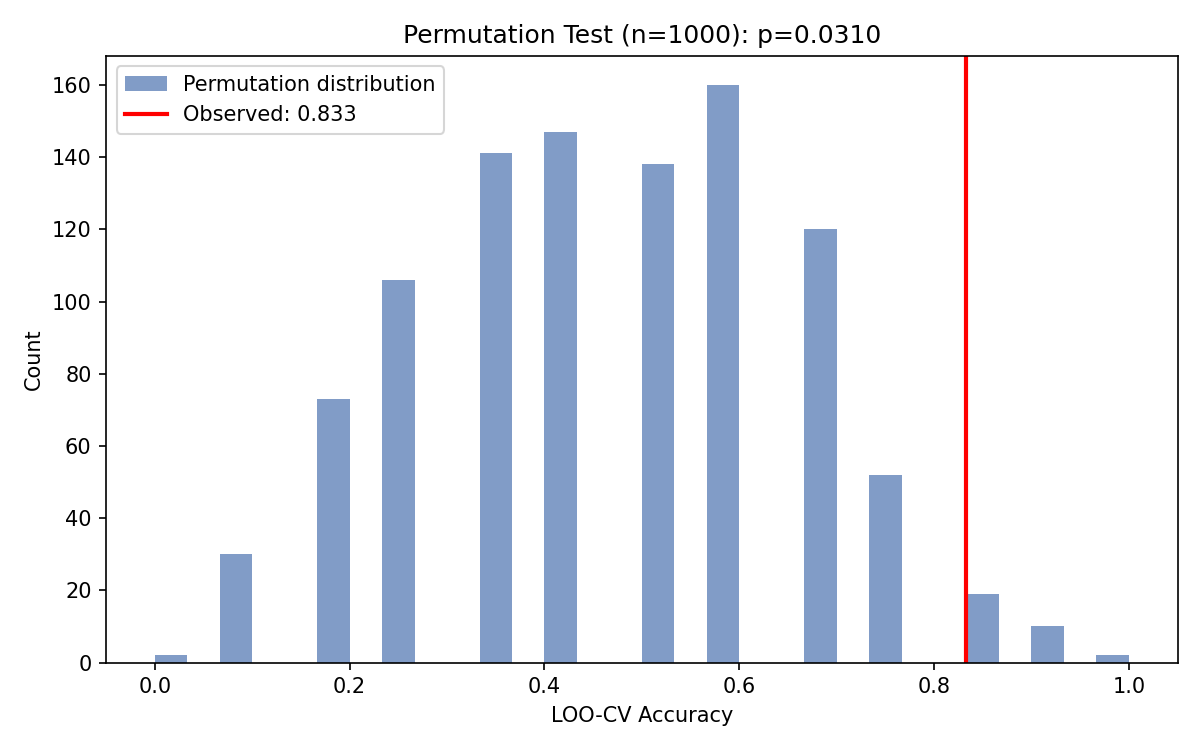
\includegraphics[width=\columnwidth]{figures/fig3_permutation_test.png}
\caption{Figure 3: Permutation test null distribution}
\label{fig:fig3_permutation_test}
\end{figure}

\textbf{Figure 3}: Permutation test results (n=1000 shuffles). Observed LOO-CV accuracy of 83.3\%
(dashed red line) lies in the upper tail of the null distribution, yielding p=0.031 (one-tailed).

\textbf{Sensitivity analysis:} LOO-CV accuracy is 83.3\% at k=1, 75.0\% at k=3, and 66.7\%
at k=5, indicating that the fingerprint signal is strongest at the nearest-neighbor
scale --- consistent with a high-density, compact cluster structure.

\begin{figure}[htbp]
\centering
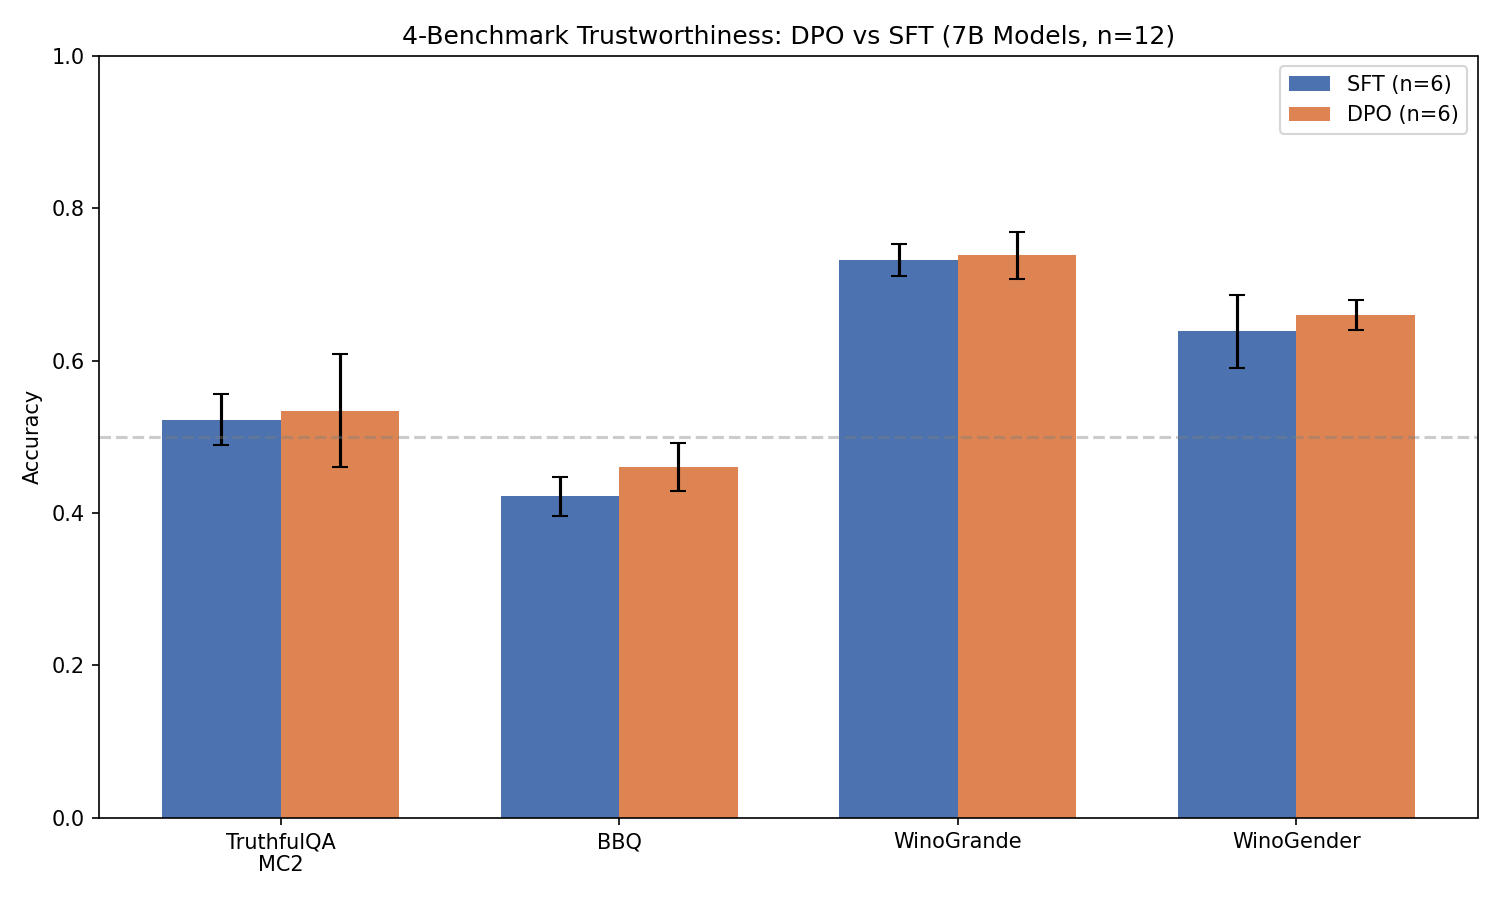
\includegraphics[width=\columnwidth]{figures/fig1_benchmark_comparison.png}
\caption{Figure 1: Group mean benchmark scores}
\label{fig:fig1_benchmark_comparison}
\end{figure}

\textbf{Figure 1} (DPO: blue, SFT: orange): Group mean benchmark scores ($\pm std)$ for DPO and SFT
models across all four evaluation tasks. DPO models score higher on TruthfulQA MC2
(+4.6pp per-pair mean) while differences on BBQ, WinoGrande, and WinoGender are small
and inconsistent across pairs.

\textbf{Table 5: $12\times 4$ benchmark score matrix.}

\begin{table*}[htbp]
\centering
\resizebox{\dimexpr 2\columnwidth+\columnsep\relax}{!}{%
\begin{tabular}{llllll}
\toprule
Model & Alignment & TruthfulQA MC2 & BBQ & WinoGrande & WinoGender \\
\midrule
Mistral-7B-Instruct-v0.1 & SFT & 0.559 & 0.430 & 0.750 & 0.550 \\
zephyr-7b-alpha & SFT & 0.549 & 0.380 & 0.730 & 0.650 \\
OpenHermes-2.5-Mistral-7B & SFT & 0.492 & 0.450 & 0.740 & 0.710 \\
tulu-2-7b & SFT & 0.482 & 0.450 & 0.710 & 0.630 \\
Llama-2-7b-chat (RLHF) & SFT* & 0.495 & 0.420 & 0.700 & 0.660 \\
Mistral-7B-Instruct-v0.3 & SFT & 0.559 & 0.400 & 0.760 & 0.630 \\
**SFT Mean** &  & **0.523** & **0.422** & **0.732** & **0.638** \\
zephyr-7b-beta & DPO & 0.514 & 0.390 & 0.690 & 0.650 \\
tulu-2-dpo-7b & DPO & 0.578 & 0.470 & 0.710 & 0.630 \\
openchat\_3.5 & DPO & 0.447 & 0.480 & 0.770 & 0.670 \\
Starling-LM-7B-alpha & DPO & 0.437 & 0.480 & 0.770 & 0.690 \\
neural-chat-7b-v3-1 & DPO & 0.592 & 0.470 & 0.760 & 0.670 \\
neural-chat-7b-v3-3 & DPO & 0.638 & 0.470 & 0.730 & 0.650 \\
**DPO Mean** &  & **0.534** & **0.460** & **0.738** & **0.660** \\
\bottomrule
\end{tabular}
}
\end{table*}

*Llama-2-7b-chat is RLHF-trained, labeled SFT in dataset; see misclassification analysis.

\begin{figure}[htbp]
\centering
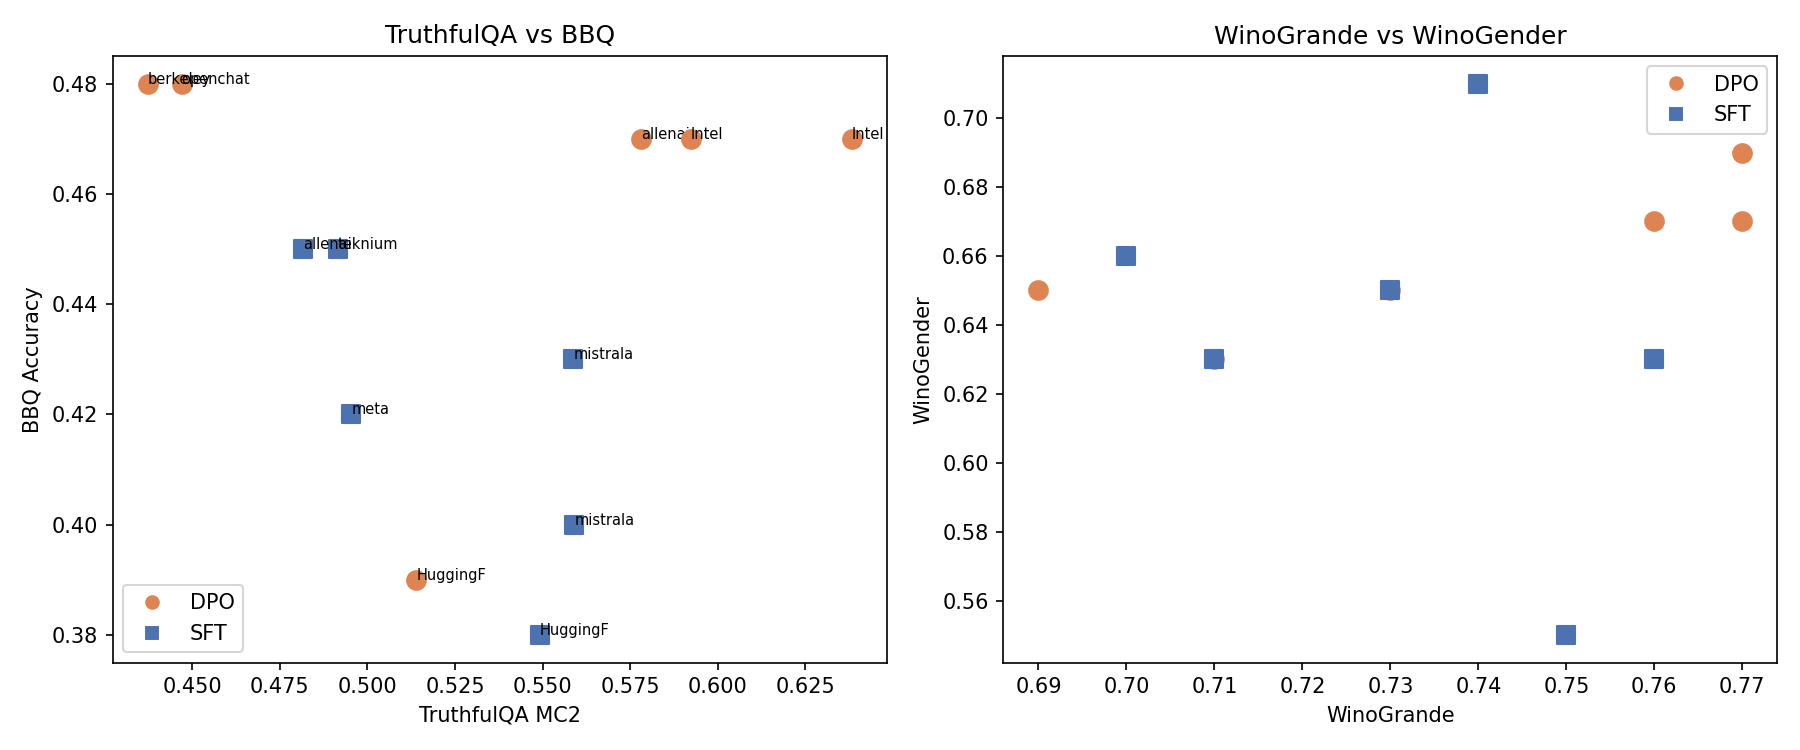
\includegraphics[width=\columnwidth]{figures/fig2_scatter_2d.png}
\caption{Figure 2: 2D score space projections}
\label{fig:fig2_scatter_2d}
\end{figure}

\textbf{Figure 2} (DPO: blue, SFT: orange): 2D projections of the 4D benchmark score space
($TruthfulQA\times BBQ$ left; $WinoGrande\times WinoGender$ right). DPO and SFT models cluster separately
in TruthfulQA-anchored projections. Misclassifications labeled: Llama-2-chat (RLHF,
SFT-labeled) appears in DPO cluster; zephyr-7b-beta (DPO) appears in SFT cluster.

Two models are misclassified (2/12):

\textbf{Case 1: Llama-2-7b-chat (RLHF $\rightarrow$ classified DPO).} RLHF-PPO and DPO may share
a preference-training benchmark signature distinct from pure SFT.

\textbf{Case 2: zephyr-7b-beta (DPO $\rightarrow$ classified SFT).} Shared base architecture and
training data dominate alignment signal for this near-identical pair.

\subsubsection{5.2 RQ2: Discriminative Dimensions and Mechanism (h-m1)}

\textbf{The fairness-advantage mechanism is refuted; truthfulness is the dominant discriminative dimension.}

\begin{figure}[htbp]
\centering
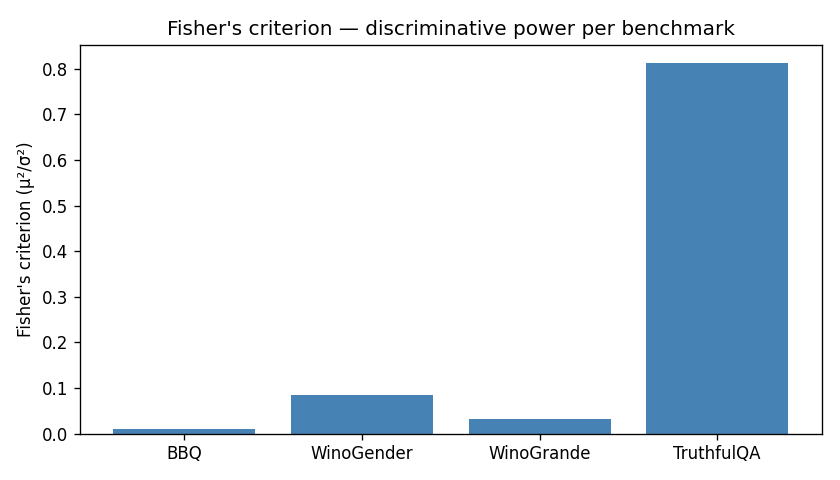
\includegraphics[width=\columnwidth]{figures/fig3_fisher_criterion.png}
\caption{Figure 6: Fisher's criterion per benchmark}
\label{fig:fig3_fisher_criterion}
\end{figure}

\textbf{Figure 6} (from h-m1/figures/fig3\_fisher\_criterion.png): Fisher's criterion (class
separability) for each of the four benchmark dimensions. TruthfulQA MC2 dominates
(Fisher=0.8122), exceeding the next highest dimension (WinoGender=0.0856) by 9.$5\times$.
BBQ provides essentially no discriminative signal (Fisher=0.0091).

\begin{table}[htbp]
\centering
\resizebox{\columnwidth}{!}{%
\begin{tabular}{llll}
\toprule
Benchmark & Fisher's Criterion & Rank & Predicted Rank \\
\midrule
TruthfulQA MC2 & **0.8122** & 1 & 3 (neutral) \\
WinoGender & 0.0856 & 2 & 1 (high) \\
WinoGrande & 0.0312 & 3 & 4 (neutral) \\
BBQ & 0.0091 & 4 & 1 (high) \\
\bottomrule
\end{tabular}
}
\end{table}

\textbf{Table 6: Fisher's criterion per benchmark.}

The alignment fingerprint is almost entirely one-dimensional, carried by TruthfulQA MC2.
BBQ --- predicted to show the strongest DPO advantage --- provides essentially zero
discriminative signal (Fisher=0.0091). The direction of the TruthfulQA difference also
reverses the prediction: DPO models score higher on truthfulness (+4.6pp per-pair mean delta),
whereas the mechanism predicted neutral-to-lower DPO truthfulness.

\textbf{BBQ fairness null result.} Although DPO models have higher mean BBQ score across the
full sample (+3.8pp group mean; Table 5: DPO mean=0.460 vs SFT mean=0.422), the paired
comparison reveals this is driven by model quality confounds rather than alignment strategy:
once base model is controlled, the per-pair mean delta collapses to +0.5pp with k=3/6 pairs
showing DPO advantage (p=0.66). This discrepancy between the group-mean difference (+3.8pp)
and the paired difference (+0.5pp) underscores the importance of the paired design for
isolating alignment effects from model-quality variation.

\begin{figure}[htbp]
\centering
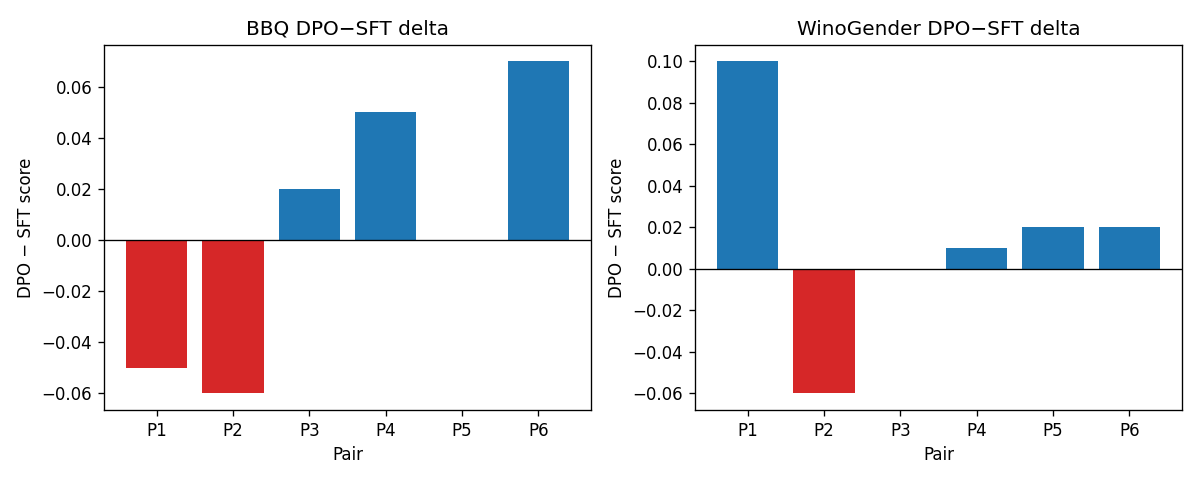
\includegraphics[width=\columnwidth]{figures/fig1_bbq_winogender_paired_bar.png}
\caption{Figure 4: Signed per-pair BBQ and WinoGender deltas}
\label{fig:fig1_bbq_winogender_paired_bar}
\end{figure}

\textbf{Figure 4}: Signed per-pair deltas (DPO score minus SFT score) for BBQ (left) and
WinoGender (right) across all 6 model pairs. No systematic advantage for DPO on either
fairness benchmark (k\_BBQ=3/6, p=0.66; k\_WinoGender=4/6, p=0.34).

\begin{table}[htbp]
\centering
\resizebox{\columnwidth}{!}{%
\begin{tabular}{llll}
\toprule
Metric & Value & Threshold & Status \\
\midrule
k\_BBQ (DPO>SFT pairs) & 3/6 & $\geq 4$ & FAIL \\
p\_BBQ (one-sided binomial) & 0.6562 & $\leq 0.125$ & FAIL \\
k\_WinoGender & 4/6 & --- & (p=0.34) \\
mean\_BBQ\_delta & +0.005 & --- & vs +0.046 TruthfulQA \\
\bottomrule
\end{tabular}
}
\end{table}

\textbf{Table 7: h-m1 gate results.}

\begin{figure}[htbp]
\centering
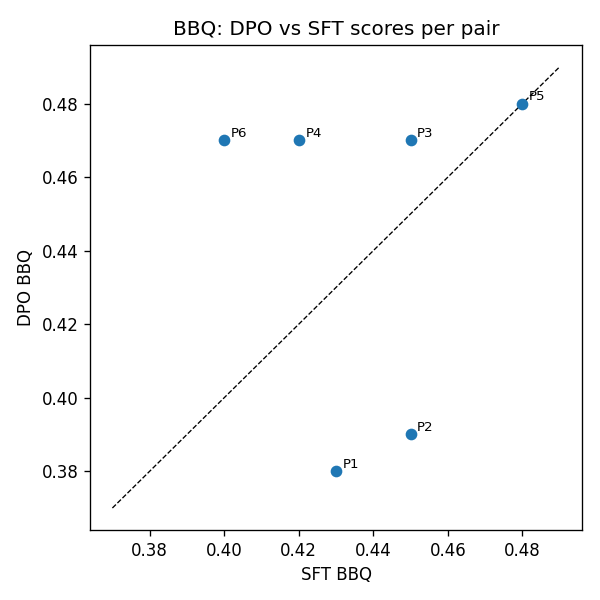
\includegraphics[width=\columnwidth]{figures/fig2_bbq_scatter.png}
\caption{Figure 5: BBQ per-pair scatter}
\label{fig:fig2_bbq_scatter}
\end{figure}

\textbf{Figure 5}: Scatter plot of BBQ scores for each model pair (DPO score vs SFT score).
Points near the diagonal indicate no systematic advantage. Three of six pairs fall above
(DPO>SFT); three fall below.

\begin{figure}[htbp]
\centering
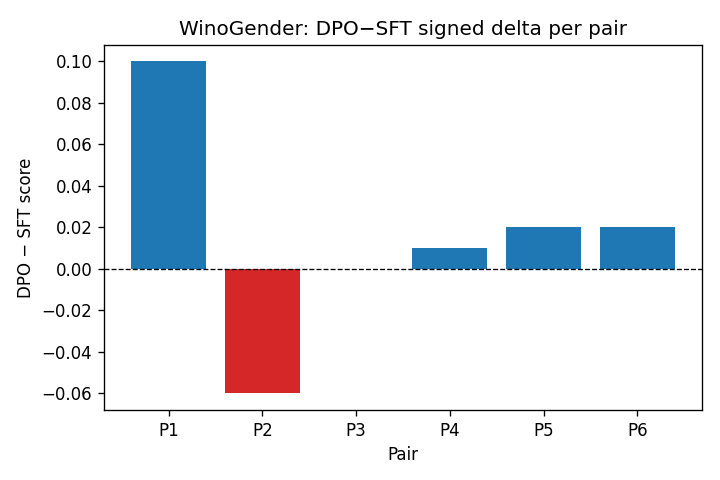
\includegraphics[width=\columnwidth]{figures/fig4_winogender_delta.png}
\caption{Figure 7: WinoGender per-pair deltas}
\label{fig:fig4_winogender_delta}
\end{figure}

\textbf{Figure 7}: Signed WinoGender deltas per model pair (DPO minus SFT). No systematic
DPO advantage observed (k=4/6, p=0.34).

\textbf{Summary:} The fingerprint exists (RQ1: PASS) but operates through an unexpected
mechanism (RQ2: fairness hypothesis refuted). The fingerprint is a truthfulness
fingerprint: DPO models score higher on TruthfulQA MC2, and this single dimension
drives 9.$5\times$ more separability signal than any fairness benchmark.

